\chapter*{Anexo II: Uso en docencia}
\label{cap:anexoii}

\noindent En este anexo se aborda el cómo se pretende incluir este robot en la asignatura de Robótica Industrial del Grado de Robótica Software 
de la Universidad Rey Juan Carlos. Primeramente, 
se ha consultado con Julio Lora, actual profesor de esta asignatura, cómo se podría integrar este trabajo en el siguiente curso académico. Se llegó 
a la conclusión de que una buena manera de utilizar este robot en sus clases, sería para complementar al robot UR3, utilizado actualmente 
para enseñar a los alumnos a generar trayectorias de soldadura. Teniendo además el punto fuerte de aprender a programar un brazo robot a través de un framework 
de código abierto como es MoveIt2. En base a lo anterior, se ha planteado un posible ejercicio práctico.

\section*{Ejercicio: Ejecutando trayectorias en MoveIt 2}
\noindent Crear un programa en Python para que el robot G-Arm ejecute una trayectoria con framework de MoveIt2. La trayectoria debe consistir 
en una lista de puntos de paso. Además, se debe hacer uso de la herramienta \textit{Porta lápices} para dibujar la trayectoria sobre un folio 
con el robot real. 

\subsection*{Competencias adquiridas}
\noindent Al realizar este ejercicio los alumnos aprenderán las siguientes competencias:
\begin{enumerate}
    \item Conocer la existencia del framework de MoveIt.
    \item Aprender a generar los puntos de paso de distintas figuras.
    \item Controlar y programar un brazo robot mediante la API de Python de MoveIt2.
    \item Representar el recorrido de un eslabón con Rviz.    
\end{enumerate}

\newpage
\subsection*{Conocimientos necesarios para resolverlo}
\noindent Para solucionar el ejercicio propuesto, es necesario conocer las herramientas disponibles. Una de ellas es librería PyMoveIt2, 
la cuál proporciona una serie de clases y métodos que facilitan la interación con este framework. Dentro de ella, existen una serie de clases 
que nos permiten controlar el robot de las siguientes formas:
\begin{enumerate}
\item \textbf{\textit{Joint goal}}: Permite controlar el robot en el espacio de articulaciones, es decir llevar cada articulación del robot a posición angular concreta.
\item \textbf{\textit{Pose goal}}: Permite controlar el robot en el espacio cartesiano, es decir llevar al extremo del robot a una posición XYZ con una 
cierta orientación.
\item \textbf{\textit{Gripper action}}: Permite interactuar con la herramienta del robot a través de una serie de cómodas funciones.
\item \textbf{\textit{Servo}}: Permite mandar comandos en tiempo real (sin la previa planificación que requieren los anteriores) para controlar las velocidad lineares y 
angulares del extremo del robot.

\end{enumerate}

Como en este caso se pretenden realizar trayectorias, es necesario utilizar las funciones relativas a \textbf{\textit{Pose goal}}.


\subsection*{Desarollo de la solución}
\noindent Primeramente, se ha creado un programa sencillo en Python con cuatro funciones las cuales devuelven una lista de puntos que corresponden 
con los vértices de cuatro figuras: cuadrado, círculo, tríangulo y un corazón. Para comprobar que los puntos son correctos, se puede utilizar la librería 
Turtle para dibujarlos. Por otro lado, es necesario implementar un bucle que itere sobre la lista de puntos y mueva el robot hasta el siguiente. Para hacer 
esto, es necesario crear una instancia de la clase \textit{MoveIt2} y utilizar los métodos \textit{move\_to\_pose()} y \textit{wait\_until\_executed()} 
como se muestra en el fragmento de código \ref{code:pymoveit2_ex1}.
\begin{code}[ht!]
\begin{lstlisting}[language=Python,  literate={á}{{\'a}}1 {é}{{\'e}}1 {í}{{\'i}}1 {ó}{{\'o}}1 {ú}{{\'u}}1 {ñ}{{\~n}}1, commentstyle=\color{gray}]
    
from pymoveit2 import MoveIt2

# Object creation
moveit2 = MoveIt2(
    node=self._node,
    joint_names=g_arm.joint_names(),
    base_link_name=g_arm.base_link_name(),
    end_effector_name=g_arm.end_effector_name(),
    group_name=g_arm.MOVE_GROUP_ARM,
    callback_group=callback_group,
    follow_joint_trajectory_action_name="/arm_controller/follow_joint_trajectory",
    execute_via_moveit=False
)

# Target position related to frame_id variable
position = (0.25, 0.0, 0.0) 

moveit2.move_to_pose(position=position, quat_xyzw=(1.0, 0.0, 0.0, 0.0), cartesian=True, 
                    frame_id=g_arm.base_link_name(), target_link=g_arm.end_effector_name(), tolerance_orientation=3.14)

# Wait until there is no action running                  
moveit2.wait_until_executed()

\end{lstlisting}
\caption{Uso básico de PyMoveIt2 para moverse a un punto}
\label{code:pymoveit2_ex1}
\end{code}

\newpage
El código completo de la solución se encuentra, junto al resto de ejemplos, en el repositorio de github del 
proyecto\footnote{\url{https://github.com/RoboticsURJC/tfg-vperez/blob/main/src/software/g\_arm\_python_examples/g\_arm_python\_examples/trajectory.py}}. Para 
probarlo, debemos ejecutar lo siguiente (cada comando en una terminal distinta):
\begin{verbatim}
    ros2 launch g_arm_moveit2 show_end_effector_travel.launch 
    ros2 run g_arm_python_examples trajectory
\end{verbatim}

\newpage
Para visualizar el recorrido de un determinado eslabón se debe de activar la opción \textit{Show Trail} de \textit{RobotModel}. En este caso, interesa activar la 
del extremo del robot, como se muestra en la Figura \ref{fig:activarTrail}.
\begin{figure} [ht!]
    \begin{center}
        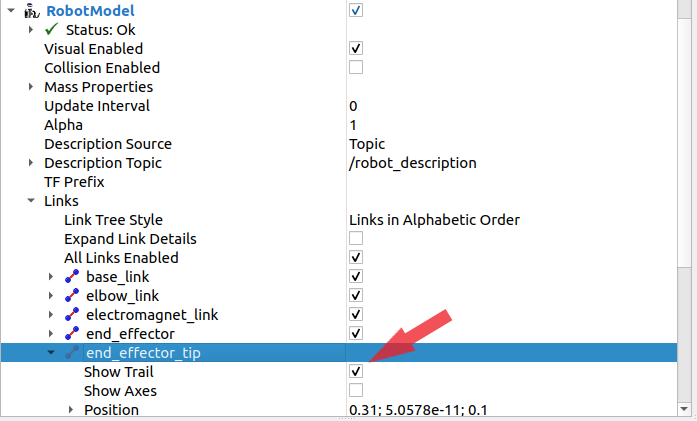
\includegraphics[width=11cm]{figs/rviz_show_trail.png}
    \end{center}
    \caption{Activación de la opción Show Trail de un link en Rviz}
\label{fig:activarTrail}
\end{figure}

En la Figura \ref{fig:trayectorias} se puede ver las distintas trayectorias de ejemplo ejecutadas .

\begin{figure} [ht!]
    \centering  
    \subfigure[Cuadrado]{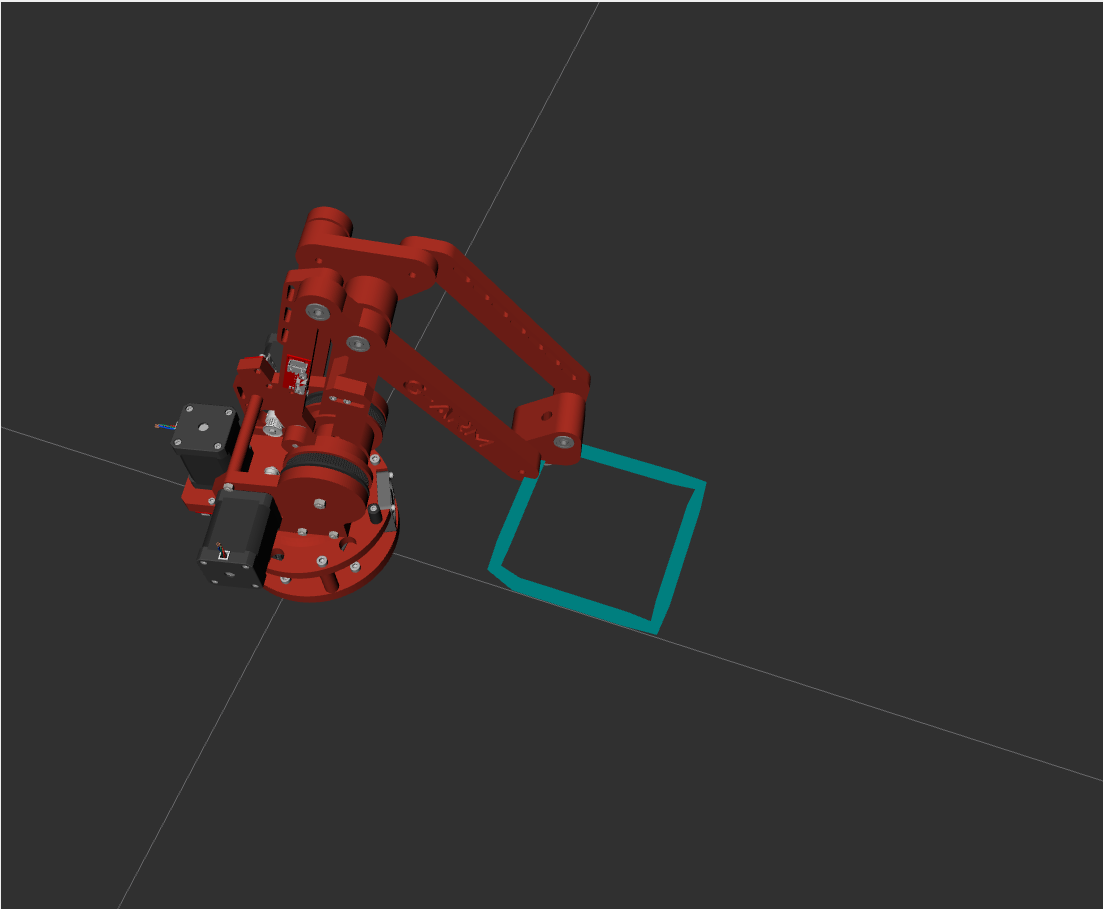
\includegraphics[width=0.35\linewidth ]{figs/square.png}}
    \hspace{2cm}
    \subfigure[Círculo]{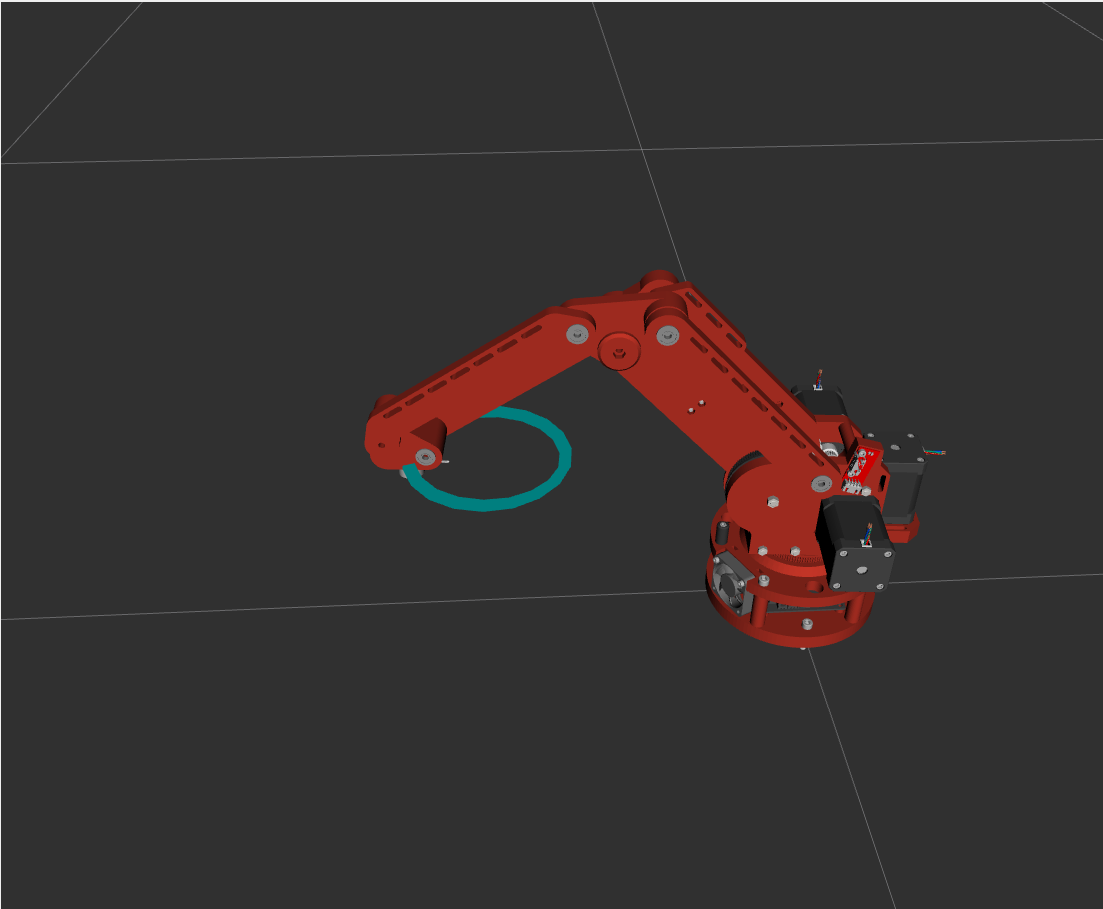
\includegraphics[width=0.35\linewidth ]{figs/circle.png}}
    \hspace{2cm}
    \subfigure[Triángulo]{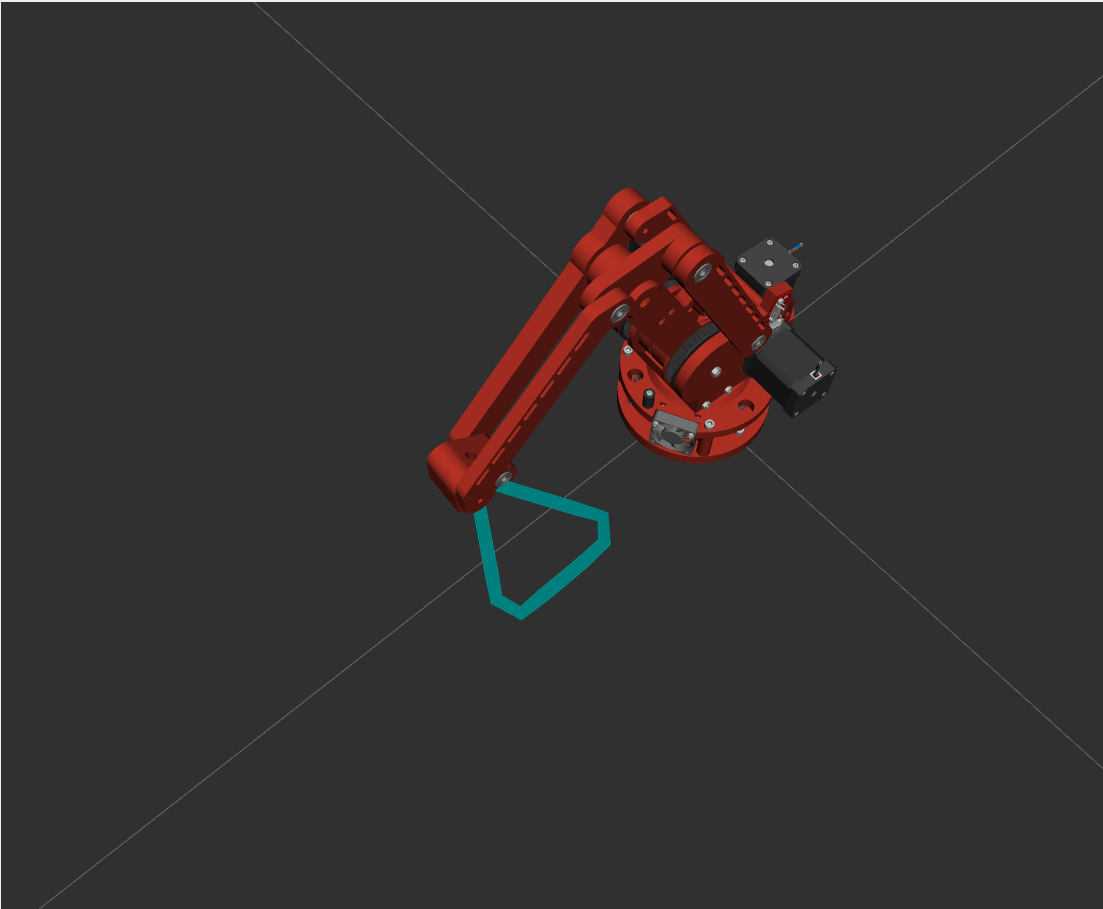
\includegraphics[width=0.35\linewidth ]{figs/triangle.png}}
    \hspace{2cm}
    \subfigure[Corazón]{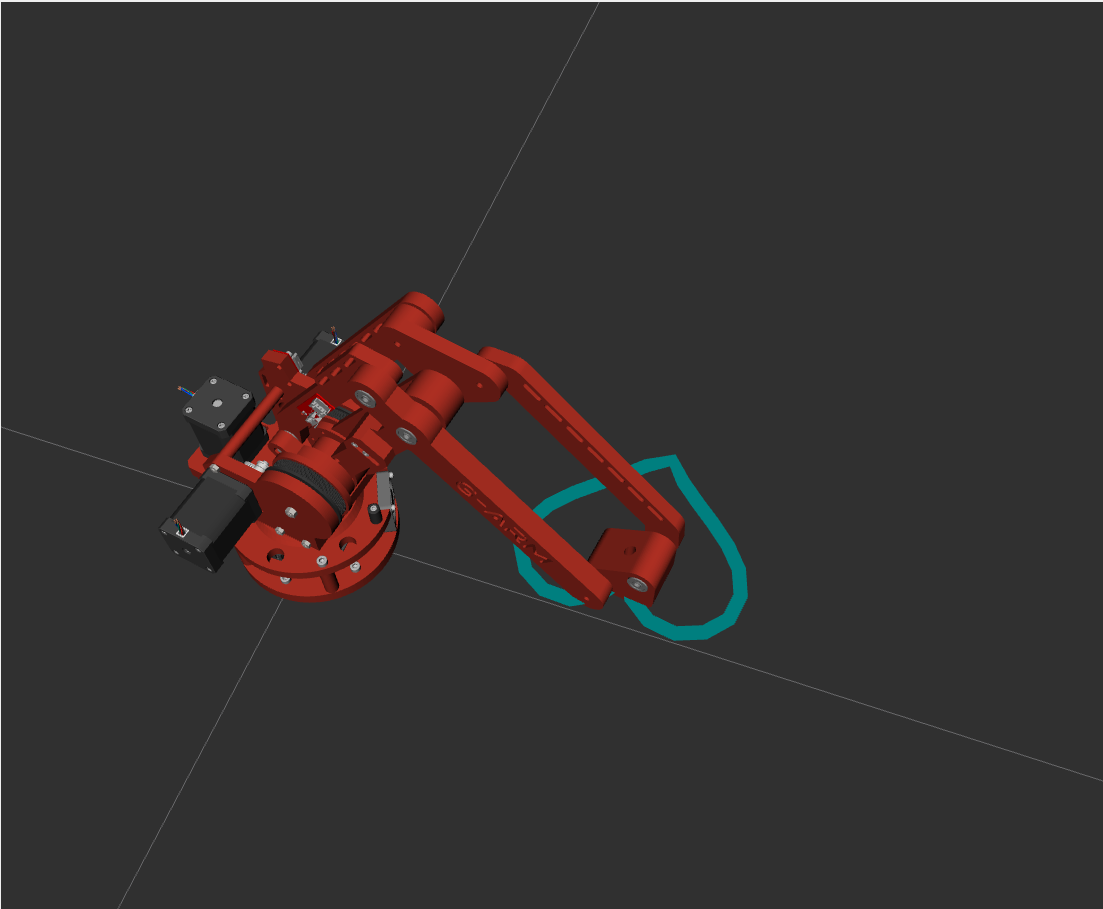
\includegraphics[width=0.35\linewidth ]{figs/heart.png}}
    \caption{Trayectorias realizadas}
    \label{fig:trayectorias}
\end{figure}\ 

Finalmente, con el objetivo de probar la trayectoria en el robot real, se ha diseñado una herramienta nueva (Figura \ref{fig:pen_tool}). Se trata de un porta lápices que utiliza la 
flexión del PLA para acoplar un lápiz al extremo del robot de una forma robusta y sin holguras, siendo a su vez flexible. Se puede descargar el modelo 
desde la carpeta de piezas del repositorio (24\_TOOL\_Pen.FCStd).
\begin{figure} [ht!]
    \centering  
    \subfigure[Vista lateral]{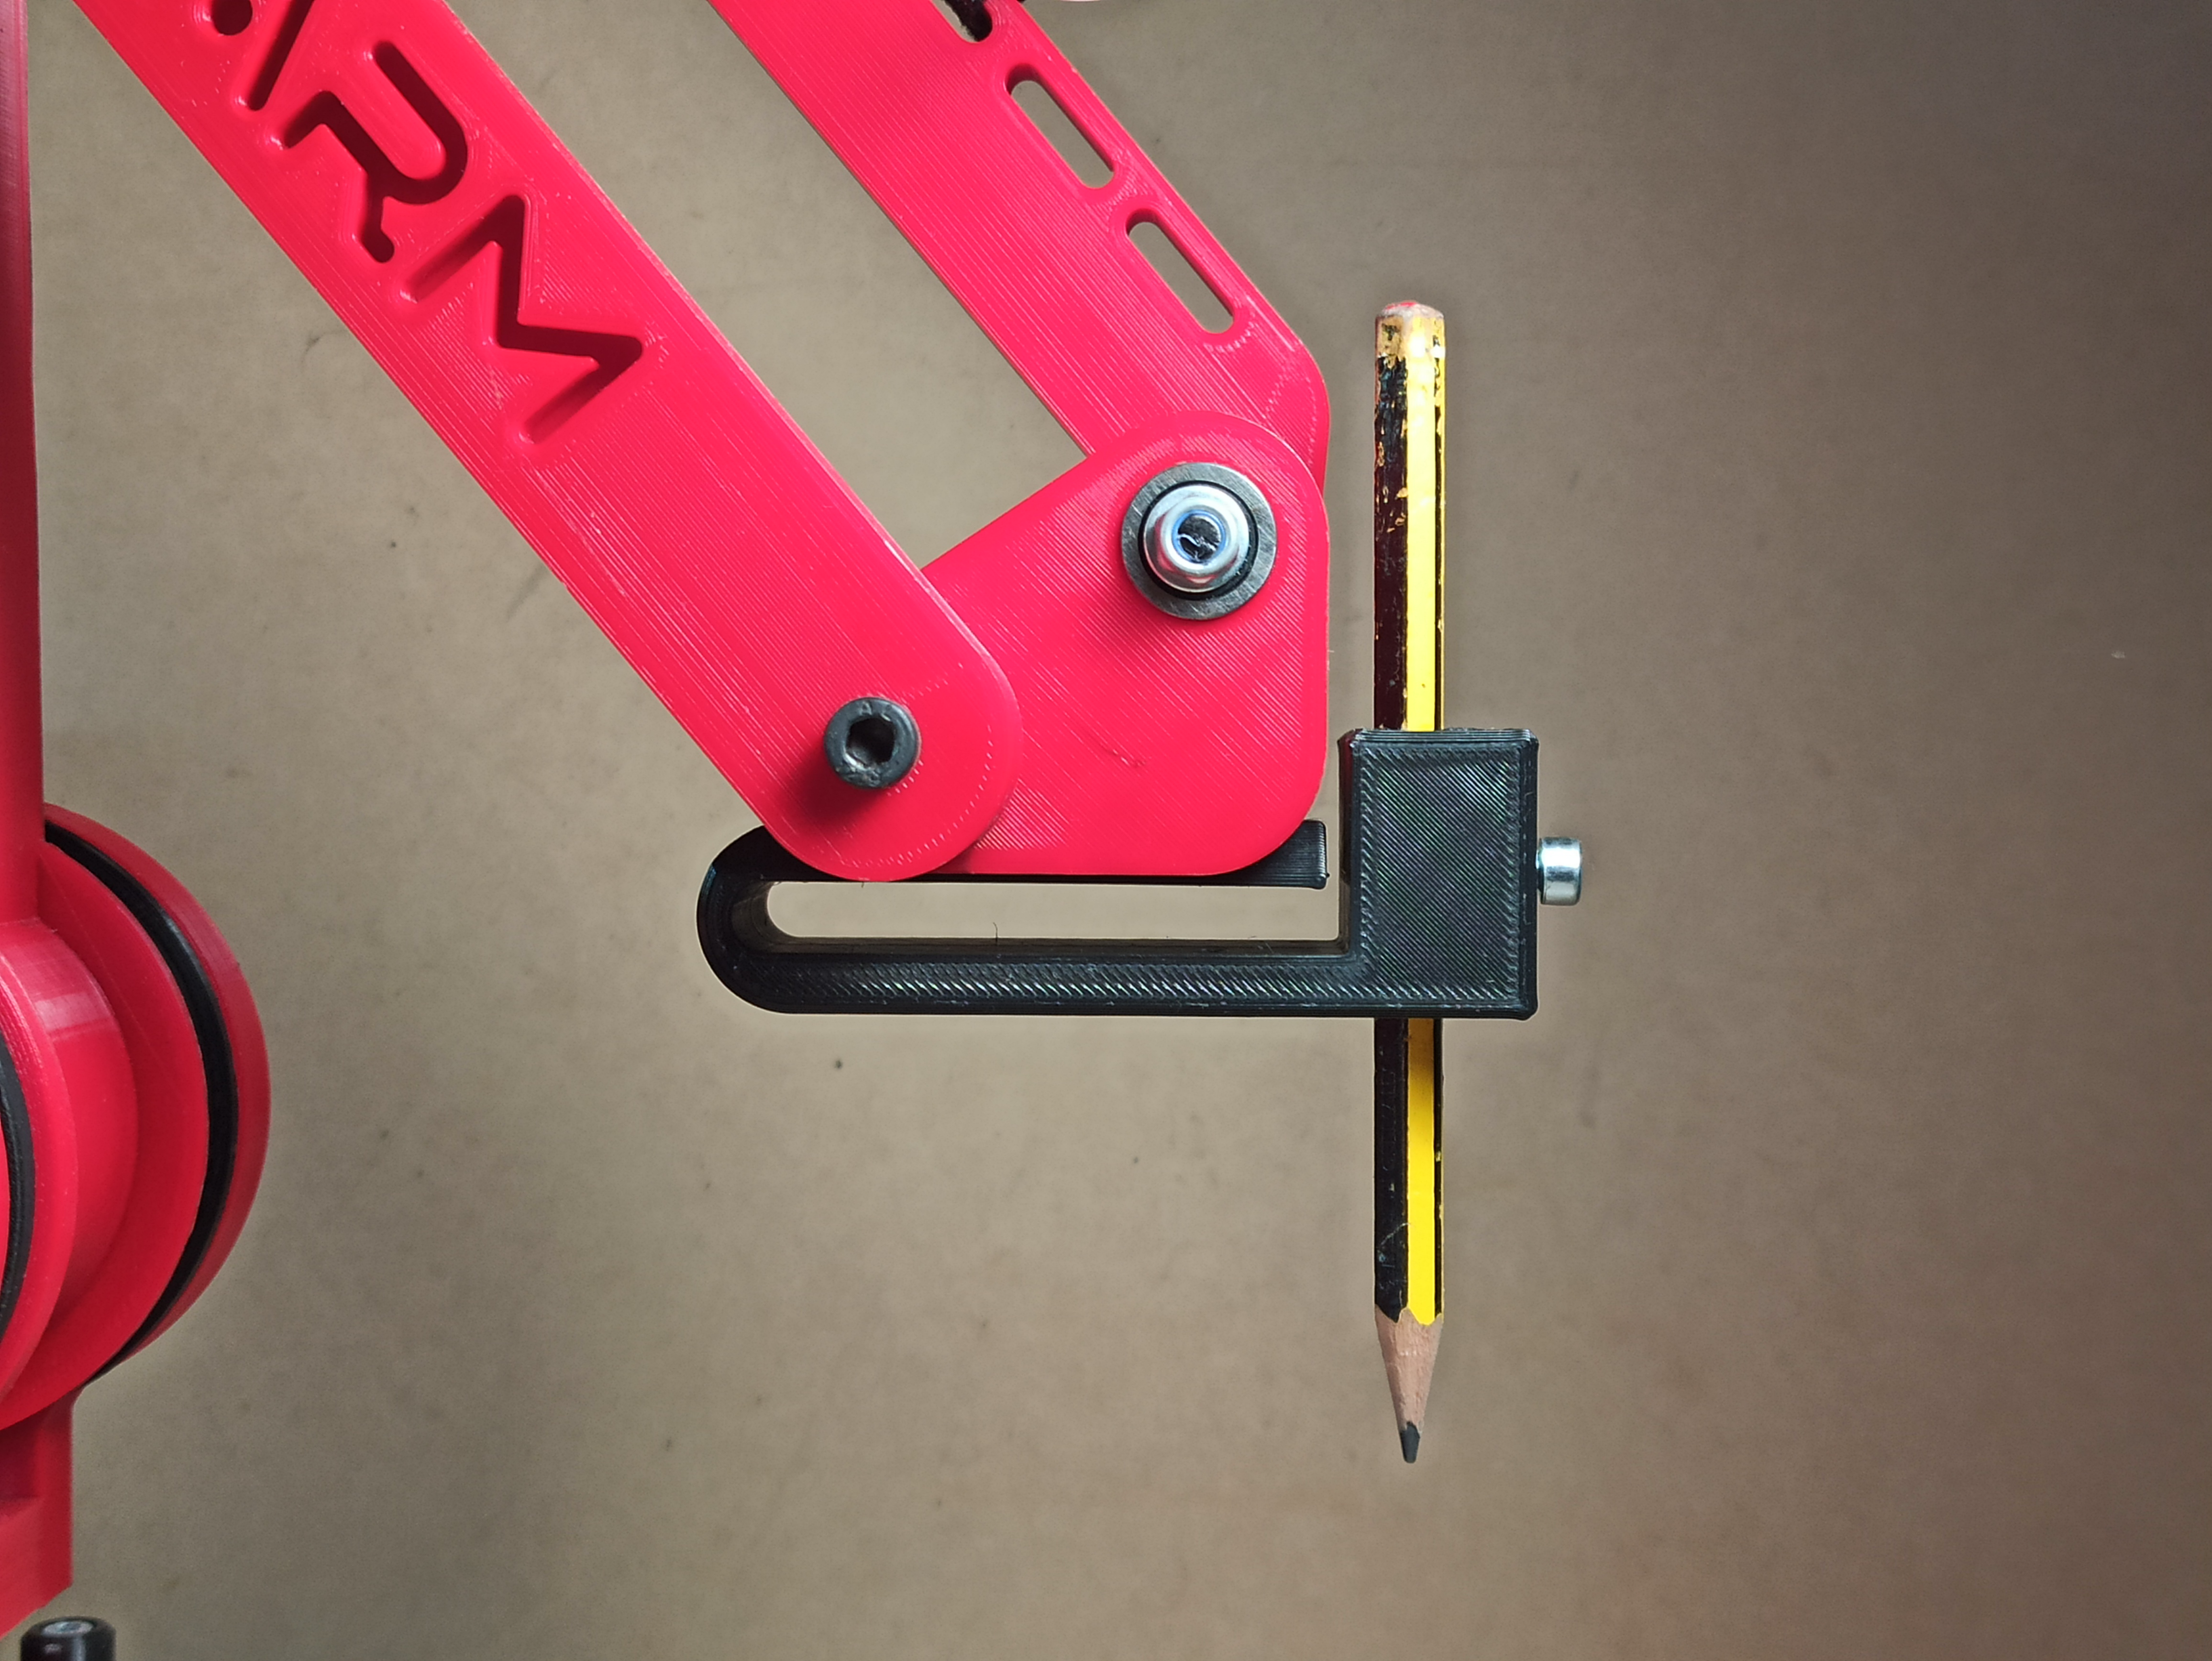
\includegraphics[width=0.6\linewidth ]{figs/pen_tool.jpg}}
    \hspace{1cm}
    \subfigure[Vista completa]{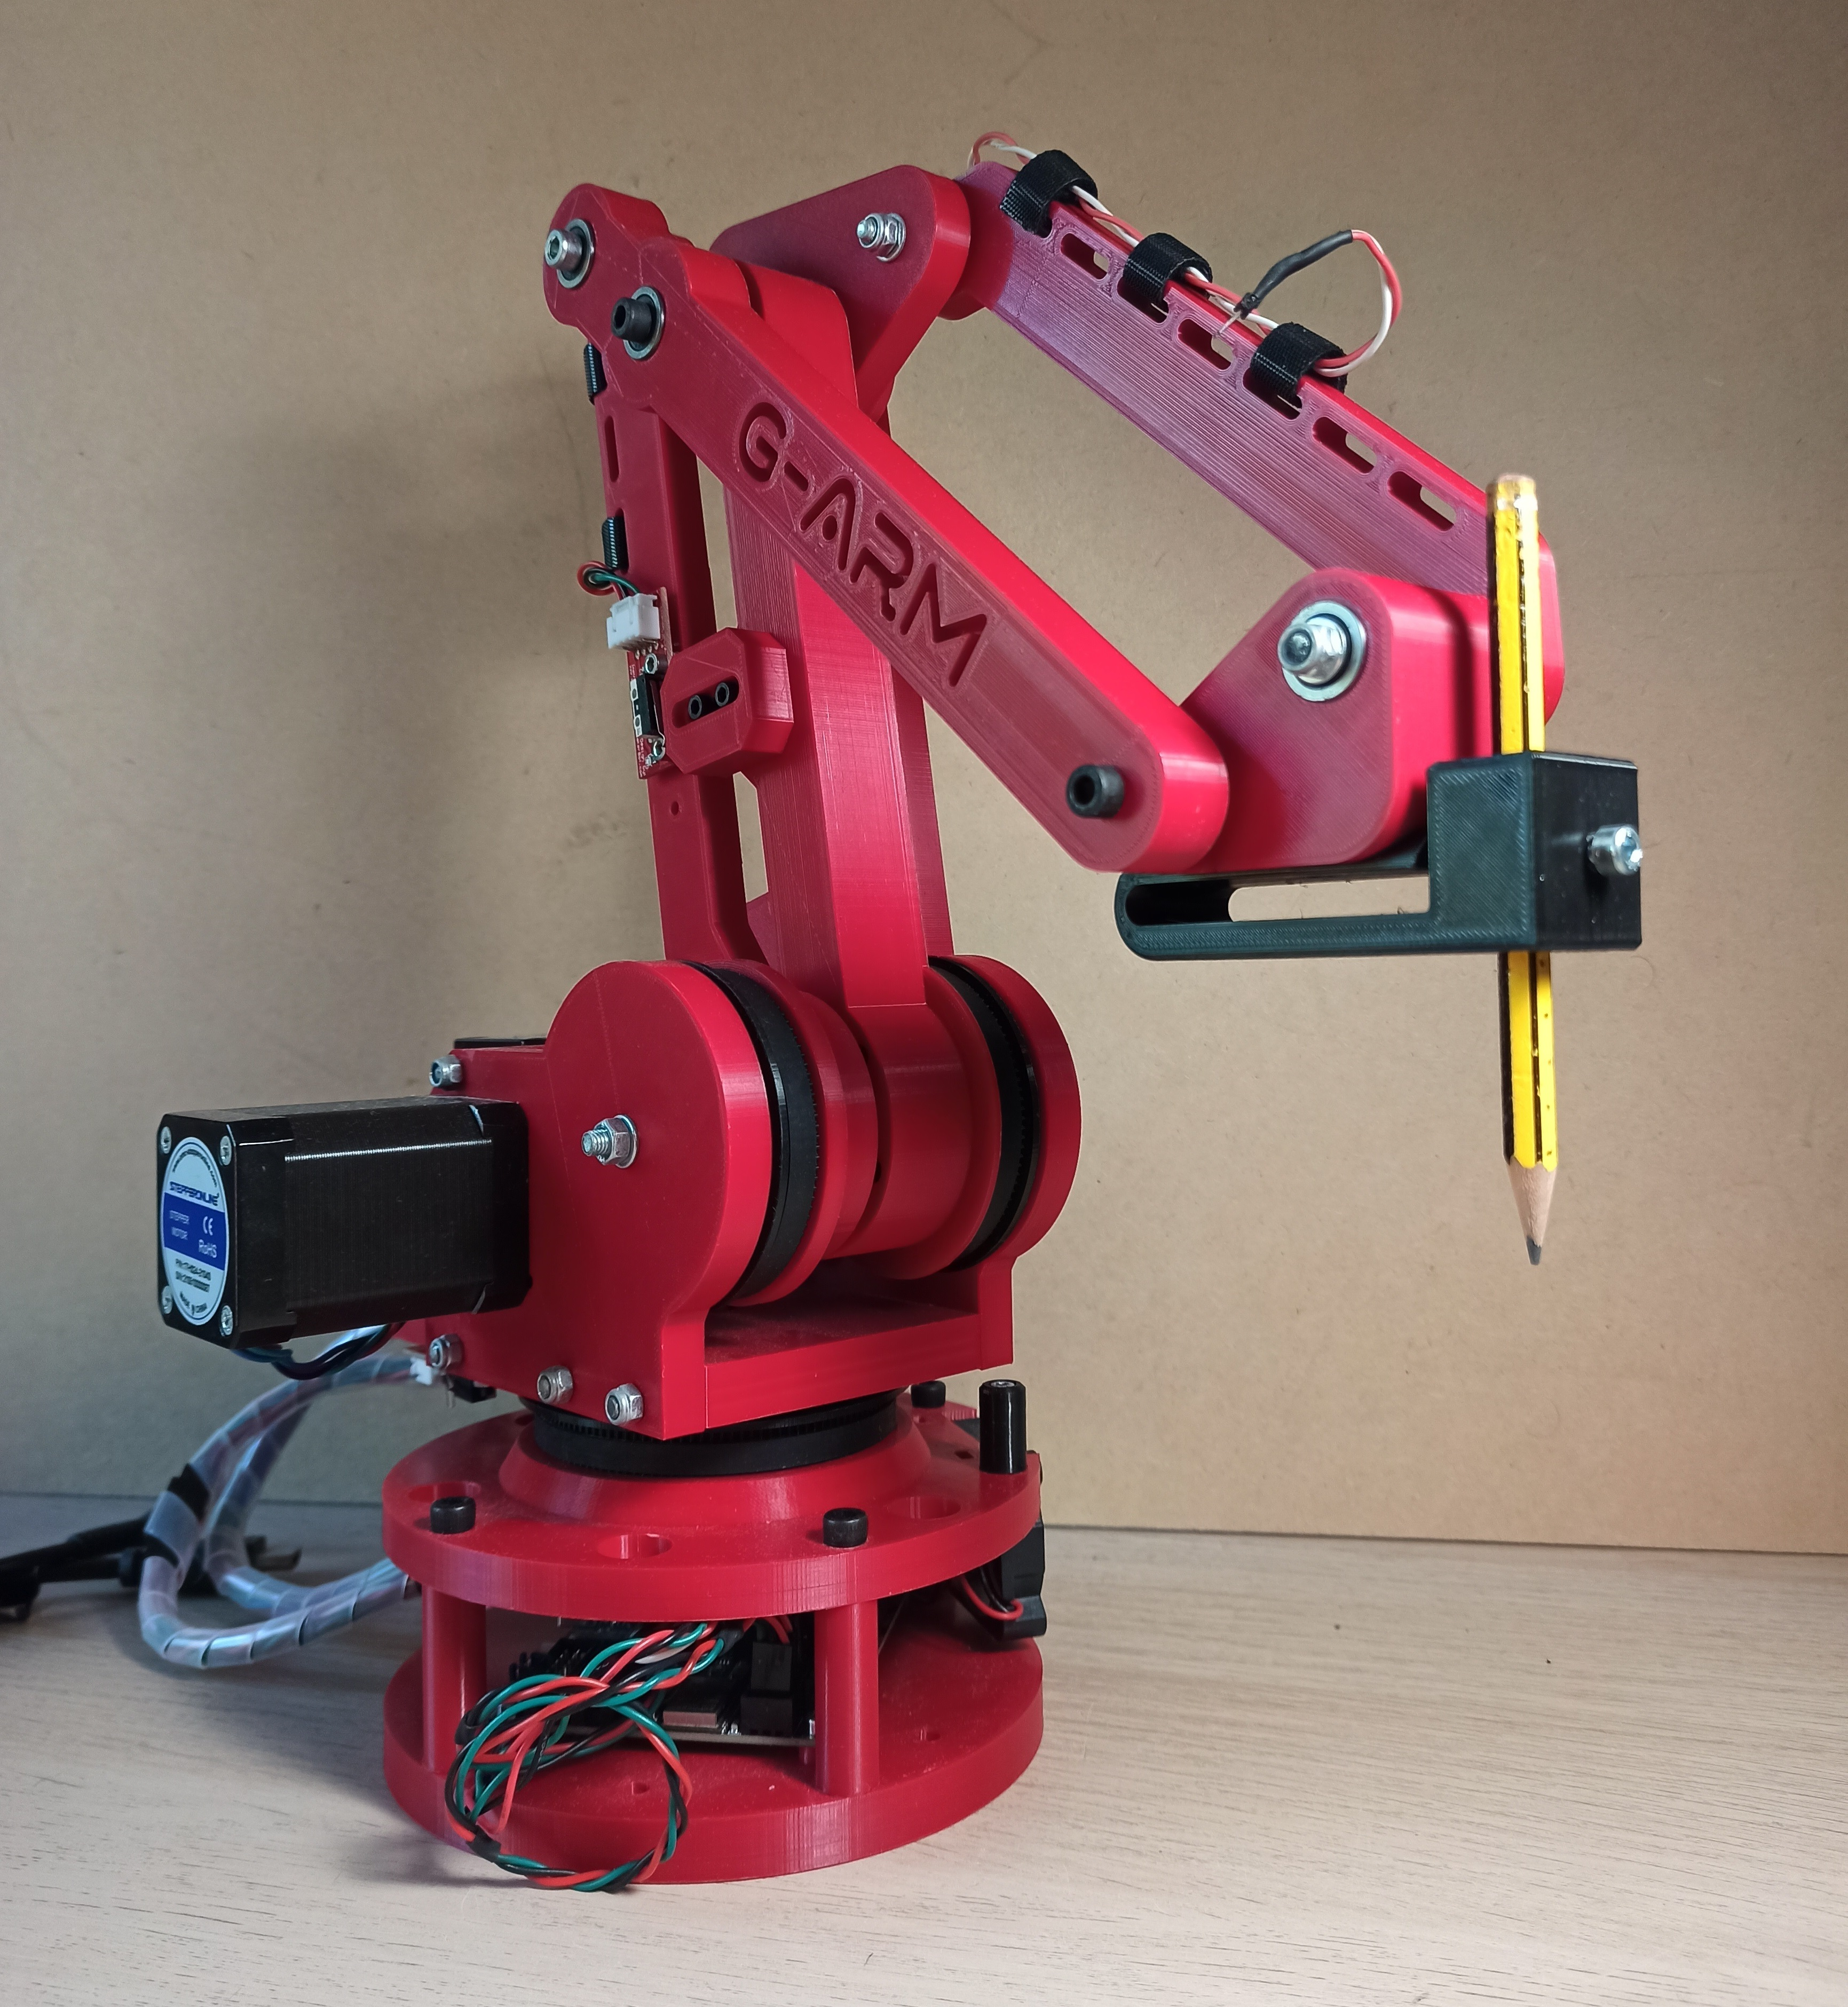
\includegraphics[width=0.6\linewidth ]{figs/robot_with_pen.jpg}}
    \caption{Herramienta porta lápices}
    \label{fig:pen_tool}
\end{figure}\ 
\newpage
Se ha escogido un plano con una altura en Z igual a 10cm, ya que en este plano es capaz de alcanzar una gran cantidad de puntos. En él, se ha dispuesto 
una base plana y un folio en el que se ha dibujado la figura más compleja del ejemplo, el corazón. El resultado de todo el proceso de dibujado puede verse en el siguiente 
vídeo\footnote{\url{https://youtube.com/shorts/3rwK_FV3eSs}}. Adicionalmente, en la Figura \ref{fig:real_draw} se muestra algunas imágenes extraídas de él.
\begin{figure} [ht!]
    \centering  
    \subfigure[Durante la trayectoria]{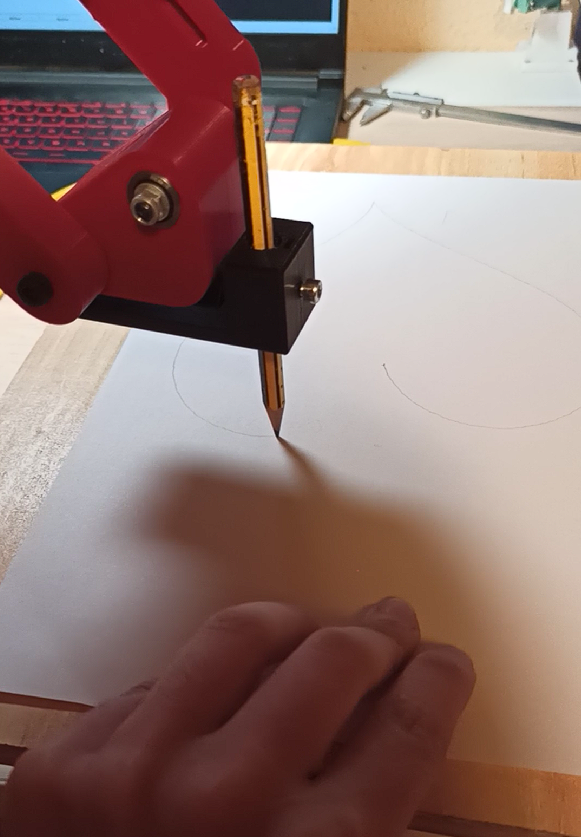
\includegraphics[width=0.41\linewidth ]{figs/drawing.png}}
    \hspace{1cm}
    \subfigure[Resultado final]{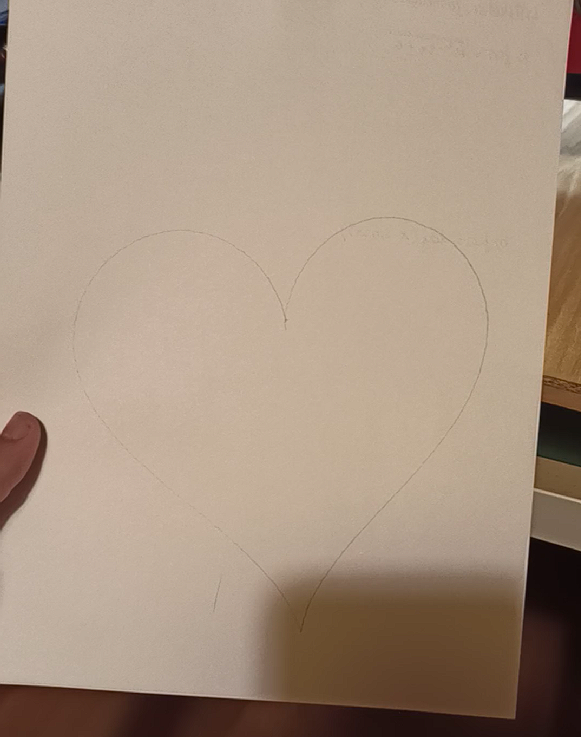
\includegraphics[width=0.46\linewidth ]{figs/drawing_result.png}}
    \caption{Prueba en el robot real}
    \label{fig:real_draw}
\end{figure}\ 

Como se puede ver, el trazado es excelente, por lo que puede ser utilizado para realizar todo tipo de trayectorias asegurando unos buenos resultados.


\newpage
\section*{Ejercicio extra: Uso de una herramienta actuada}
\noindent Crear un programa en Python para llevar a cabo una tarea de manipulación con el robot G-Arm. La tarea consiste en coger una moneda de una determinada posición y 
depositarla en otra distinta, haciendo uso de la herramienta \textit{Electroimán}.

\subsection*{Conocimientos previos}
\noindent La herramienta acoplada al robot debe ser controlada mediante un joint ficticio con un rango de movimiento de 0.0 a 1.0 radianes. Este 
valor es convertido por el driver de ROS en un valor entendible por la salida PWM del extremo del robot. En la configuración del paquete de MoveIt se 
estableció que este joint no pertenece a la cadena cinemática del brazo y no es usado a la hora de planificar. Este, se controla separadamente 
en un grupo separado llamado Tool. Para controlar el actuador del extremo del robot, la librería PyMoveit2 incorpora una clase llamada \textit{MoveIt2Gripper} y principalmente dos 
funciones: \textit{open()} y \textit{close()}.

\subsection*{Desarrollo}
\noindent En este ejercicio se ha utilizado la clase \textit{MoveIt2Gripper} mencionada anteriormente, tal y como 
se muestra en el fragmento de código \ref{code:pymoveit2_ex2}.
\begin{code}[ht!]
\begin{lstlisting}[language=Python,  literate={á}{{\'a}}1 {é}{{\'e}}1 {í}{{\'i}}1 {ó}{{\'o}}1 {ú}{{\'u}}1 {ñ}{{\~n}}1, commentstyle=\color{gray}]
# Create MoveIt 2 gripper interface
tool = MoveIt2Gripper(
node=self._node,
gripper_joint_names=g_arm.tool_joint_name(),
open_gripper_joint_positions=g_arm.electromagnet_on(),
closed_gripper_joint_positions=g_arm.electromagnet_off(),
gripper_group_name=g_arm.MOVE_GROUP_GRIPPER,
follow_joint_trajectory_action_name="/tool_controller/follow_joint_trajectory",
callback_group=callback_group)

tool.open() # Open gripper (electromagnet on)
tool.wait_until_executed()
tool.close() # Close gripper (electromagnet off)
tool.wait_until_executed()
\end{lstlisting}
\caption{Uso básico de PyMoveIt2 para moverse a un punto}
\label{code:pymoveit2_ex2}
\end{code}
\newpage
Posteriormente, se han establecido una serie de puntos: P0, PA1, PA2, PB1, PB2 (Figura \ref{fig:example_electromagnet_2}). Y se ha utilizado 
los conocimientos del anterior ejercicio para moverse entre ellos.
\begin{figure} [ht!]
    \begin{center}
        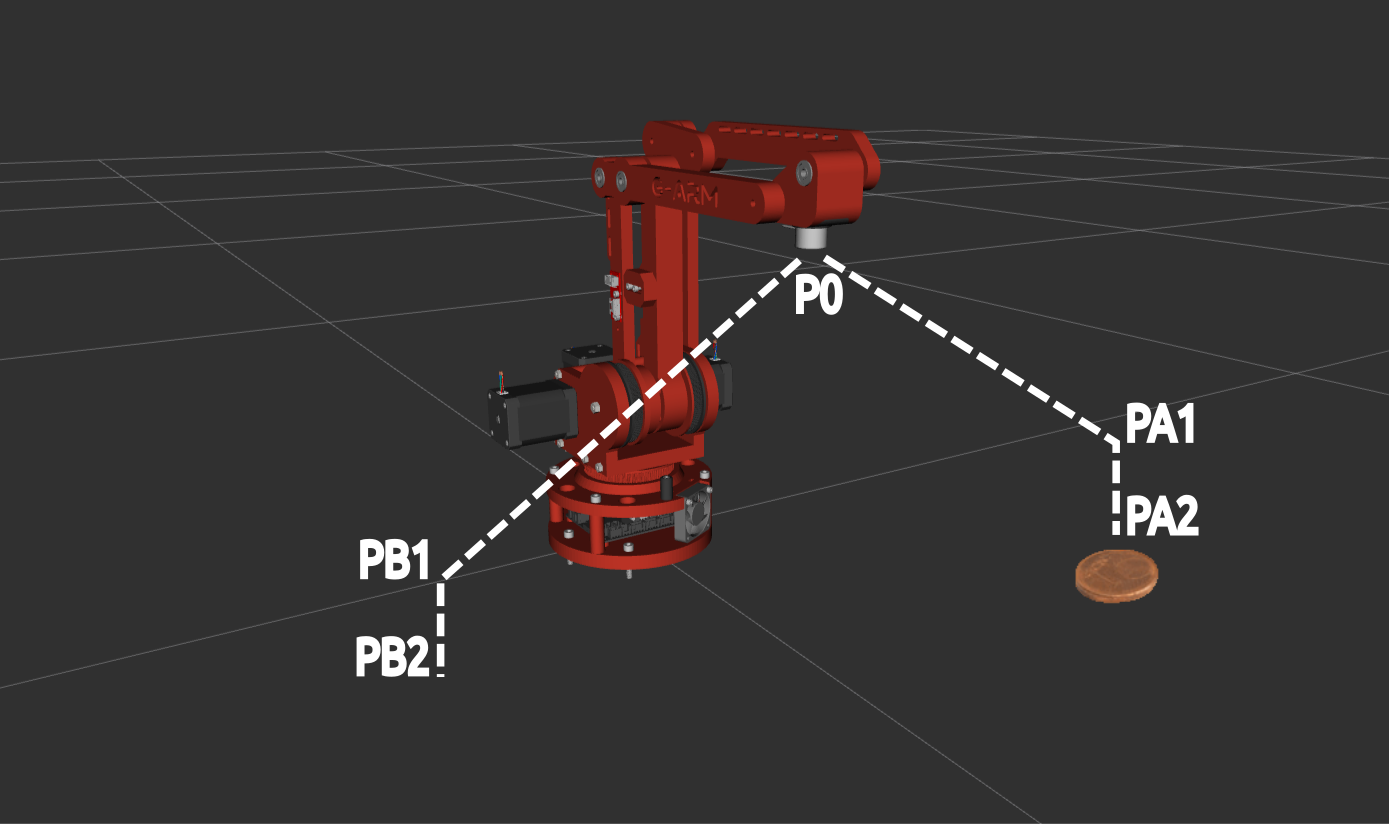
\includegraphics[width=12cm]{figs/ex2.png}
    \end{center}
    \caption{Puntos del ejercicio}
\label{fig:example_electromagnet_2}
\end{figure}


El código completo de la solución se encuentra, junto al resto de ejemplos, en el repositorio de github del 
proyecto\footnote{\url{https://github.com/RoboticsURJC/tfg-vperez/blob/main/src/software/g\_arm\_python_examples/g\_arm_python\_examples/electromagnet.py}}. Para 
probarlo, debemos ejecutar lo siguiente (cada comando en una terminal distinta):
\begin{verbatim}
    ros2 launch g_arm_moveit2 show_end_effector_travel.launch 
    ros2 run g_arm_python_examples electromagnet
\end{verbatim}
En este enlace\footnote{\url{https://youtu.be/iRcEg6AgwcU}} se puede ver el vídeo que se ha grabado de la ejecución en el robot real.